% Technical Background, section 2 (drafted 2026-11-06 as 08_fpca.tex; moved 2026-11-07 from
%   thesis/technical_background/04_fpca.tex, text unchanged).
% 2026-11-07: Sangalli's classification result (21.5% leave-one-out error, K chosen on the same
%   data) moved to the Literature Review (sec:lit-measure).
% 2026-11-08: rewritten after wang2016fda, read in full as arXiv:1507.05135 (skill fpca-wang holds
%   the claim check). Single-source rule (root CLAUDE.md): every general FPCA statement cites
%   wang2016fda alone; ramsay2005fda is no longer cited in this file. Changes:
%   - CUT (user, 2026-11-08; thesis-style: no individual studies in the Technical Background): the
%     Sangalli 2009 AneuRisk paragraph (65 patients, 33.4% / 18.2%; it stays in sec:lit-measure) and
%     the Warmenhoven 2021 result (39 children, R^2 = 0.99). Replaced by the paragraph on mapping
%     each segment onto [0, 1] as a landmark registration.
%   - CUT: the sentence on nearly equal eigenvalues being unstable (no source found).
%   - FIXED against Wang: alpha "usually up to 2" (not "1 or 2"); no 80 or 90% thresholds (Wang
%     calls scree and FVE ad hoc, gives no numbers); "BIC selects fewer than AIC" (not "information
%     criteria select fewer"); grid estimation as sample mean, covariance and a matrix
%     eigenproblem (Wang pp. 5, 9).
%   - UNCITED on purpose, as derivation: the rectangle rule, the scaling factors in
%     eq:tech-fpca-grid, the sequential reading of the eigenfunctions, the sign argument, and
%     "specific to the sample, domain and preprocessing".
%   - NEW CITE: outcome-blind components (Wang p. 26).
%   - sangalli2009aneurisk dropped from the non-identifiability sentence (Wang covers it).
% 2026-11-08 (second pass, after outdated/thesis_retired/style_guide_technical_aida.md): definition
%   opener restored ("FPCA is a ... designed for ..., where ..."); origin sentence added (1940s-50s,
%   inference framework 1970s; Wang p. 8, dates only, no names); "scores" glossed once, at
%   eq:tech-fpca-score (was glossed twice); appositive "each the pair of ..." made its own clause;
%   defining property stated as such; grid step phrased as a reduction under the rectangle rule;
%   hazard closer split into Aida's two sentences ("Correct ... depends on ... Otherwise, ...") and
%   made general ("a vessel segment"), so the Methodology makes the link. No tool paragraph: the
%   software is a setting and stays in Methods 07.
% 2026-11-08 (third pass, user): opener rebuilt as a middle way between the problem-first and the
%   definition-first versions. "Samples of curves" now explained after Wang p. 2 ("for each subject
%   ... one or several functions are recorded"; "curve data"): one function per subject, the whole
%   function is the observation. Sentence 2 shortened (no repeated "regression model"); history cut
%   to one clause (1970s inference framework, Wang p. 8), the 1940s-50s origin dropped as unused.
% 2026-11-08 (fourth pass, user: "optimise for easy understanding on the first read, less clunky"):
%   prose rewritten for readability, with claims, citations, equations and labels unchanged.
%   Long nominal sentences split; intuition before the formal statement (eigenfunctions read one
%   by one, scores read by sign, the expansion as "adding the shapes back"); the vascular sentence
%   moved up to the third sentence of the opener, so "curve" is concrete from the start.
% CHECK: warmenhoven2021pca is now cited only for "FPCA on an equal grid is PCA with the positions
%   as variables, by SVD"; confirm the primer states this (only its R^2 result was read).
% CHECK: marron2015amplitude full text not read; it carries amplitude/phase as terms and the
%   variance-inflation and shift-size mixing claim.
% 2026-11-09 (fifth pass, user: "use the phrases and way of explaining in the JMP guide; plain
%   language to support the math; figures where the math is hard to picture; project-specific math
%   waits until the Methodology"). Style source: Hersh P., "Understanding functional principal
%   component analysis (FPCA)", JMP web guide (PDF in the repo root). It is used for the order of
%   explanation and plain wording only and is NOT cited (vendor page; single-source rule keeps every
%   general FPCA claim on wang2016fda). Taken from it: whole curve instead of isolated points; shape,
%   not just level; interpretation starts from the mean and the deviations from it; eigenfunctions
%   read as shapes and scores as how strongly a curve shows a shape; curve = mean + score x shape,
%   shown as a picture before the Karhunen-Loeve equation; mean +/- score x shape for reading a
%   component; the scree plot as where adding components stops paying. Not taken: "dynamic data"
%   (the profiles vary along a position, not over time), basis fitting as a required step, its
%   90-99% rule for K, its claim that smoothing is built in.
%   - MERGED: the two duplicate opener paragraphs (one with a stray character) into one.
%   - MOVED to Methods 07 (sec:method-fpca, as notes): the paragraph on mapping a vessel segment
%     onto [0, 1] as landmark registration, and the respacing of the unevenly spaced centerline
%     points onto the grid. The opener no longer names curvature or radius profiles, and "bend"
%     became "feature" or "peak": this section now holds only general FPCA.
%   - NEW: five figures from made-up curves (content/technical/figures/fpca_figures.py):
%     fig:tech-fpca-curves, fig:tech-fpca-cov, fig:tech-fpca-rebuild, fig:tech-fpca-modes,
%     fig:tech-fpca-phase. The sentences that read the figures (taller peak, tilt, plateau) describe
%     the simulation, not a claim about FPCA.
%   - NEW, uncited on purpose (reasoning): "curves can differ in shape and not only in level";
%     the pointer sentence in sec:tech-fpca-grid to the Methods for curves at unequal positions.
%   - Equations, labels, notation and every wang2016fda claim are unchanged in content.
% 2026-11-09 (sixth pass, user: "restructure how FPCA is explained using more of JMP, fix all
%   problems"). Now follows the JMP guide's order: what FPCA is (components and scores) -> why not
%   the raw values (correlated neighbours; shape, not just level) -> how it differs from PCA (a
%   component is a function, not a vector of weights) -> mean function and components -> scores and
%   rebuilding a curve -> reading the components -> how many to keep -> computation -> registration
%   (JMP: alignment as preprocessing). New subsections and labels: sec:tech-fpca-components,
%   sec:tech-fpca-scores, sec:tech-fpca-reading, sec:tech-fpca-k. Equations, eq labels, notation
%   and every wang2016fda claim unchanged in content. Fixed:
%   - the user's opener "(functional components)" / "(scores)": parenthetical glosses replaced by
%     "referred to as"; "functional components" became "components", the word used everywhere else.
%   - double definitions: component and score are defined once, in the opener; the later sentences
%     give their formal meaning ("Formally, the shapes are the eigenfunctions ..."; "A component is
%     thus ..."; "Formally, the score is ...") instead of glossing them again.
%   - "relate to disease" -> "relate to an outcome" (the section is general).
%   - NEW, uncited on purpose (reasoning, after JMP): PCA components as vectors of weights versus
%     FPCA components as functions of position; "the aim is to keep the main shapes without the
%     components that mostly describe noise".
%   - NEW CITE: wavelets added to the fixed-basis list (Wang p. 9 lists spline, Fourier, wavelet).
%   - Not taken from JMP: clustering and outlier detection as applications (not used here).
% 2026-11-09 (seventh pass, user: "cut all unnecessary lines on what the method is not"). CUT:
%   "Instead of treating each measured value as an isolated point" (now stated positively); "curves
%   can also differ in shape and not only in level ..." (and "address both problems"); the ordinary
%   PCA sentence (vector of weights per variable), folded into "extends PCA ..., so each component is
%   itself a function of position"; "rather than with the curves themselves"; the fixed-basis
%   sentence (splines, Fourier, wavelets), so the optimality property now opens "The basis of FPCA
%   is estimated ..."; "without looking at any outcome" and "not by how strongly they relate to an
%   outcome". KEPT on purpose: "not a tested property of the curves" (a limit of reading components)
%   and "do not draw on the test curves" (a property of the fold-wise estimation).
% 2026-11-09 (eighth pass, user: "optimise the whole section for flow and for easy understanding
%   on the first read"). Claims, cites, equations and labels unchanged. Opener reordered as
%   definition -> curve -> problem (many correlated values) -> FPCA's answer (components, scores,
%   extension of PCA) -> scores in a regression model. Eigen paragraph: no longer says "the shapes
%   are the eigenfunctions" and "each eigenfunction is one shape" twice. "The basis of FPCA" now
%   follows from the eigenfunctions (the fixed-basis sentence that introduced "basis" was cut).
%   Long modes sentence split. Sign paragraph tied to "arbitrary sign" above; fold sentence made
%   a statement of what is done. Outcome-blind paragraph tied to the choice of K. Grid opener: two
%   overlapping sentences merged. The outlier sentence now says why (covariance = second moment).
% 2026-11-09 (ninth pass, user: "infer the Aida style guide on the full section; do not be
%   unnecessarily repetitive", outdated/thesis_retired/style_guide_technical_aida.md and
%   style_guide_aida.md). Applied: definition opener "X is a [kind] designed for [task], where ...";
%   one fact per sentence, no idea stated twice; "while/whereas" contrast pairs; subsections that
%   refine (grid, registration) open on the limitation they address; hazard closer kept; no
%   forward references (Aida §9 checklist). Repetition cut:
%   - opener (6 sentences -> 4): "a few" x3, "regression model" x2, "correlated" x2, the separate
%     curve gloss and "each component is itself a function of position" (said by "shapes").
%   - "The score of a curve on a component measures how strongly ..." (said in the opener).
%   - "so that the curve is replaced by K numbers" (said in the opener), now "where the truncation
%     replaces the curve by its first K scores"; the KL cite moved to the expansion itself.
%   - "the components are ordered by how much of the variation they describe" (said by the
%     first/second-shape sentence and lambda_1 >= lambda_2).
%   - "The deviations vary around zero, and everything that follows is computed from them" merged.
%   - "read" x3 in the modes sentence; "compared" x2 in the sign paragraph; "added component" x3.
%   FORWARD REFERENCE dropped: (Section~\ref{sec:method-fpca}) in sec:tech-fpca-grid, per Aida (the
%   background never mentions the Methodology; Methods 07 points back to sec:tech-fpca-grid).
% Pointed back to by: content/methodology/07_curvature_fpca.tex (sec:method-fpca), which also takes
%   the landmark reading of the segment ends and the respacing onto the grid.
% Terms (fpca-wang section 2): "curve" is the observation, "profile" says what it measures, "bend"
%   is only the shape of the vessel. "Score" is xi_ik, "component" the pair (phi_k, lambda_k).
% Notation: x_i(t), t in [0,1], mu, Gamma, phi_k, lambda_k, xi_ik, grid t_g (g = 1..G), D, d_i,
%   v_k, w, alpha. Avoids j, s, S, b, beta, c (taken by the GLMM, the curvature section and the
%   centerline).
% LEFT OUT on purpose (Methodology): the grid size, interpolation, the 5 mm chord, the sliding
%   profile, the K rule, the segments analysed, the sign convention chosen, software.
% All cite keys are in refs.bib (added and checked on Crossref 2026-11-06).
% wordlist.txt lacks: FPCA, eigenfunction(s), Karhunen, Loeve, realizations may need checking.
% Figures: made-up curves only, from content/technical/figures/fpca_figures.py (re-run to rebuild).
% Never a Medis or tracer figure here.

\section{Functional Principal Component Analysis}
\label{sec:tech-fpca}

Functional principal component analysis (FPCA) is a dimension reduction method designed for functional data, where each observation is a whole function, referred to as a curve \cite{wang2016fda}.
A curve is recorded at many positions whose neighboring values are strongly correlated, so entering the values one by one would give a regression model many covariates that largely repeat each other \cite{wang2016fda}.
FPCA extends principal component analysis from vectors to functions and describes the curves by the shapes along which they differ most, referred to as components \cite{wang2016fda}.
How strongly a curve shows each shape is given by its scores, which are uncorrelated and replace the values of the curve as covariates \cite{wang2016fda}.

\subsection{The Mean Function and the Components}
\label{sec:tech-fpca-components}

To compare curves position by position, a position must mean the same on every curve, so all curves are placed on one common domain.
Let $x_i(t)$, $i = 1, \dots, N$, denote curve $i$ at position $t \in [0, 1]$, where $t = 0$ is the start and $t = 1$ the end of the domain.
The curves are treated as realizations of a random function $X(t)$ with $\mathrm{E}\int_0^1 X(t)^2 \, dt < \infty$ \cite{wang2016fda}.

The starting point is the mean function $\mu(t) = \mathrm{E}\,X(t)$, which is the average curve.
FPCA describes how the individual curves deviate from it, so everything that follows is computed from the deviations $x_i(t) - \mu(t)$ (Figure~\ref{fig:tech-fpca-curves}).

\begin{figure}[tbp]
  \centering
  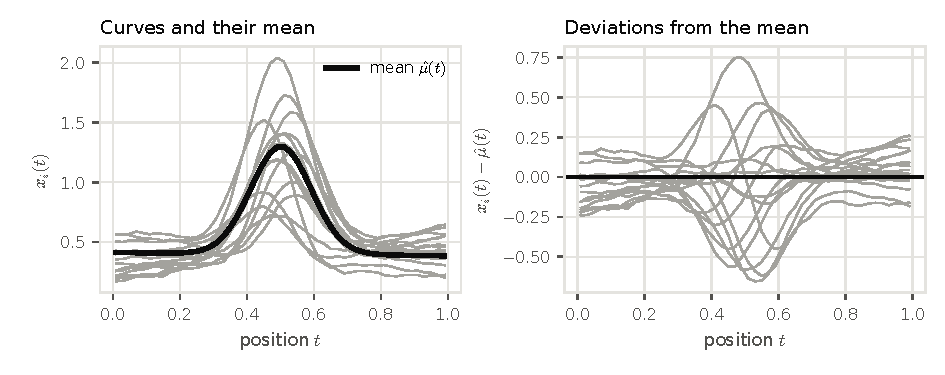
\includegraphics[width=\textwidth]{content/technical/figures/fpca_curves.pdf}
  \caption{Curves and their deviations from the mean. Left: 15 of 200 curves (grey) with their mean (black). Right: the same curves as deviations from the mean, which is what FPCA analyses. The curves are simulated and are not data from any cohort.}
  \label{fig:tech-fpca-curves}
\end{figure}

Whether the deviations at two positions tend to go together is described by the covariance function
\begin{equation}
  \Gamma(t, u) = \mathrm{cov}\{X(t), X(u)\},
  \label{eq:tech-fpca-cov}
\end{equation}
where $t, u \in [0, 1]$ are two positions on the domain.
At a single position, $\Gamma(t, t)$ is the variance of the curves there.
For two different positions, $\Gamma(t, u)$ is large when curves that lie above the mean at $t$ tend to lie above it at $u$ as well.
A feature that spreads over several neighboring positions, such as a peak whose height varies between curves, therefore shows up as a block of high covariance along the diagonal $t = u$ (Figure~\ref{fig:tech-fpca-cov}).

\begin{figure}[tbp]
  \centering
  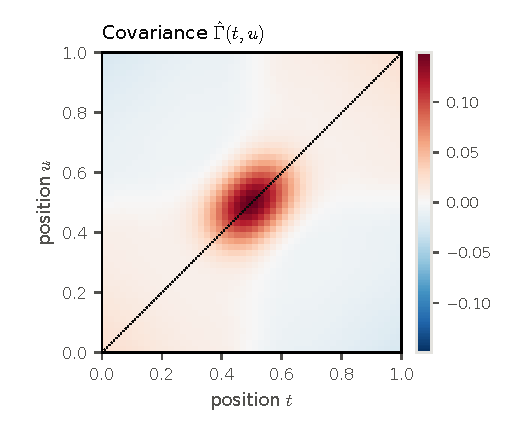
\includegraphics[width=0.55\textwidth]{content/technical/figures/fpca_covariance.pdf}
  \caption{Sample covariance function of the curves in Figure~\ref{fig:tech-fpca-curves}. Red marks pairs of positions at which the curves tend to deviate from the mean in the same direction, and the dotted line is the diagonal $t = u$, where the covariance is the variance. The block around $t = u = 0.5$ comes from the peak, whose height varies between curves at all of its positions together. The curves are simulated and are not data from any cohort.}
  \label{fig:tech-fpca-cov}
\end{figure}

The components are found by breaking this covariance down into shapes.
The first shape is the one along which the curves differ most, the second is the one along which they differ most among the shapes orthogonal to the first, and so on.
Formally, the shapes are the eigenfunctions $\phi_k$ of the covariance function, which is symmetric and non-negative definite, and each comes with an eigenvalue $\lambda_k$, so that
\begin{equation}
  \int_0^1 \Gamma(t, u)\, \phi_k(u)\, du = \lambda_k \phi_k(t),
  \qquad
  \int_0^1 \phi_k(t)\, \phi_{k'}(t)\, dt =
  \begin{cases} 1, & k = k', \\ 0, & k \neq k', \end{cases}
  \label{eq:tech-fpca-eigen}
\end{equation}
where $\lambda_1 \ge \lambda_2 \ge \dots \ge 0$ and the second condition makes the eigenfunctions orthonormal \cite{wang2016fda}.
Each eigenvalue is the variance of the curves along its eigenfunction, and the two together form a component.

\subsection{Scores and the Reconstruction of a Curve}
\label{sec:tech-fpca-scores}

A large positive score means that the curve deviates from the mean much like $\phi_k$, a large negative score means that it deviates the opposite way, and a score near zero means that the shape is nearly absent.
Formally, the score is the projection of the curve's deviation from the mean onto the eigenfunction,
\begin{equation}
  \xi_{ik} = \int_0^1 \{x_i(t) - \mu(t)\}\, \phi_k(t)\, dt ,
  \label{eq:tech-fpca-score}
\end{equation}
where $\xi_{ik}$ is the score of curve $i$ on component $k$.
The scores have mean zero and variance $\lambda_k$, and scores on different components are uncorrelated \cite{wang2016fda}.

Adding the shapes back to the mean, each weighted by its score, recovers the curve (Figure~\ref{fig:tech-fpca-rebuild}).
This is the Karhunen--Lo\`eve expansion, which in practice is truncated after $K$ terms \cite{wang2016fda},
\begin{equation}
  x_i(t) = \mu(t) + \sum_{k=1}^{\infty} \xi_{ik} \phi_k(t)
  \approx \mu(t) + \sum_{k=1}^{K} \xi_{ik} \phi_k(t),
  \label{eq:tech-fpca-kl}
\end{equation}
where the truncation replaces the curve by its first $K$ scores.
In Figure~\ref{fig:tech-fpca-rebuild}, the mean alone misses the height of the curve's peak, the first shape restores it, the second corrects the tilt along the domain, and the third adds almost nothing.

\begin{figure}[tbp]
  \centering
  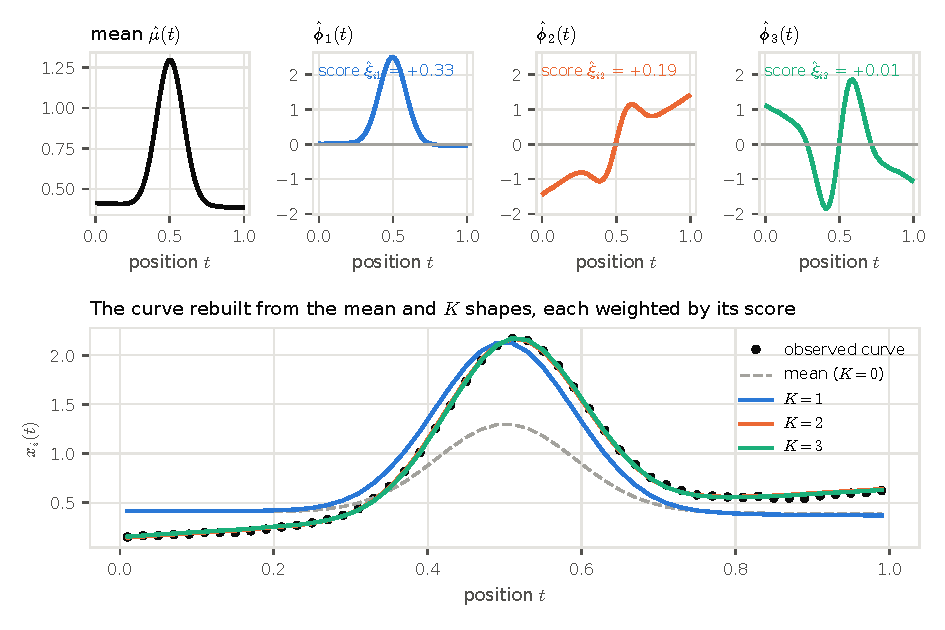
\includegraphics[width=\textwidth]{content/technical/figures/fpca_reconstruction.pdf}
  \caption{One curve rebuilt from the mean and the first three eigenfunctions. Top: the mean and the eigenfunctions, with the curve's score on each. Bottom: the observed curve (dots) and the curve rebuilt with $K = 0$ to $3$ components, each step adding one eigenfunction weighted by its score. The curves are simulated and are not data from any cohort.}
  \label{fig:tech-fpca-rebuild}
\end{figure}

The eigenfunctions thus serve as a basis for the curves, estimated from the curves themselves, and for a given $K$ no other set of $K$ basis functions approximates the curves with a smaller expected squared error \cite{wang2016fda}.
The price is that the components are specific to the sample, the domain and the preprocessing they were estimated from, so components from different samples describe different shapes.

\subsection{Reading the Components}
\label{sec:tech-fpca-reading}

An eigenfunction on its own has unit size and an arbitrary sign, so a component is shown instead by the mean together with the mean plus and minus a multiple of the eigenfunction, referred to as a mode of variation \cite{jones1992displaying, wang2016fda},
\begin{equation}
  \mu(t) \pm \alpha \sqrt{\lambda_k}\, \phi_k(t),
  \label{eq:tech-fpca-mode}
\end{equation}
where $\alpha$ usually ranges up to 2 \cite{wang2016fda}.
The curve for $+\alpha$ is the curve whose score on component $k$ lies $\alpha$ standard deviations above zero and whose other scores are all zero.
Plotted on either side of the mean, the two curves show what a high and a low score look like.
In Figure~\ref{fig:tech-fpca-modes}, a high score on the first component means a taller peak, and a high score on the second a curve that rises from the start to the end of the domain.
The name given to a component is a reading of this plot, not a tested property of the curves.

\begin{figure}[tbp]
  \centering
  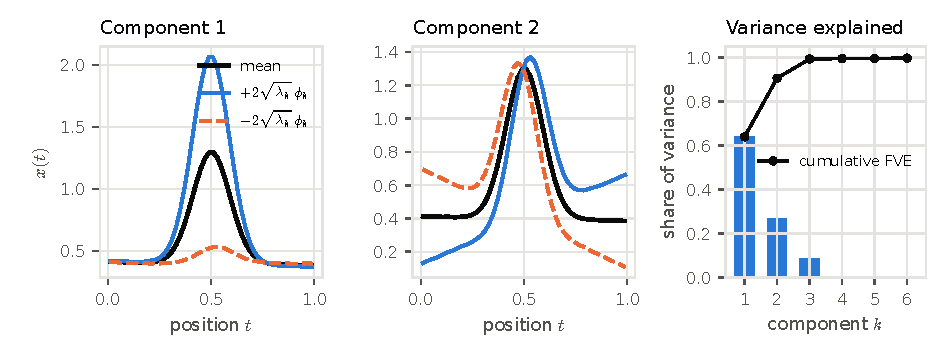
\includegraphics[width=\textwidth]{content/technical/figures/fpca_modes.pdf}
  \caption{Reading the components. Left and middle: the modes of variation of the first two components, with the mean (black) and $\mu(t) \pm 2\sqrt{\lambda_k}\,\phi_k(t)$ (colored). Right: the share of the variance per component (bars) and the cumulative fraction of variance explained (line), which levels off after three components. The curves are simulated and are not data from any cohort.}
  \label{fig:tech-fpca-modes}
\end{figure}

The arbitrary sign also matters when components are estimated more than once, since $-\phi_k$ solves Eq.~\eqref{eq:tech-fpca-eigen} whenever $\phi_k$ does, with the sign of every score $\xi_{ik}$ reversed.
A convention therefore fixes the sign, and components estimated again on bootstrap samples or cross-validation folds are aligned to it.
When the scores enter a cross-validated model, the mean and eigenfunctions are estimated within the training folds only, so the scores do not draw on the test curves.

\subsection{Choosing the Number of Components}
\label{sec:tech-fpca-k}

Each added component brings the rebuilt curves closer to the observed ones, but by less and less.
How much of the total variance the first $K$ components retain is measured by the fraction of variance explained,
\begin{equation}
  \mathrm{FVE}(K) = \frac{\sum_{k=1}^{K} \lambda_k}{\sum_{k \ge 1} \lambda_k},
  \label{eq:tech-fpca-fve}
\end{equation}
where the denominator equals $\int_0^1 \Gamma(t, t)\, dt$, the variance at each position summed over the domain.
Plotting the share of each component against $k$, referred to as a scree plot, shows where adding components stops paying (Figure~\ref{fig:tech-fpca-modes}, right).

Choosing $K$ is therefore a trade-off between keeping the main shapes and leaving out components that mostly describe noise.
A short expansion approximates the curves poorly, whereas each further component brings more estimation error, and no rule for the balance is established \cite{wang2016fda}.
The scree plot and thresholds on the fraction of variance explained are ad hoc rules carried over from ordinary principal component analysis \cite{wang2016fda}.
Of the information criteria, the Bayesian information criterion selects fewer components than the Akaike information criterion, and leave-one-curve-out cross-validation tends to select too many \cite{wang2016fda}.
Whatever the rule, it has to be fixed before the scores are related to an outcome.

The outcome plays no part in the components themselves, since FPCA builds them from the covariance of the curves alone \cite{wang2016fda}.
They are ranked by how much variance they describe, so a low-variance component can carry more information about the outcome than a leading one, and a leading one can carry none.
The covariance is a second moment, so a few outlying curves can shift its components \cite{wang2016fda}.

\subsection{Computation on a Grid}
\label{sec:tech-fpca-grid}

While FPCA is defined on continuous functions, curves are observed only at discrete points, so the integrals above cannot be evaluated directly.
When all curves are observed on one common grid of positions $t_g$, $g = 1, \dots, G$, each curve becomes a row of numbers, one per position.
The mean and covariance are then the sample mean and the sample covariance at the grid positions, and the eigenproblem becomes the eigendecomposition of a matrix \cite{wang2016fda}.
Curves observed at positions that differ between curves, or that are unevenly spaced, are first brought onto such a grid.

Let $\mathbf{D}$ be the $N \times G$ matrix with rows $\mathbf{d}_i$ and entries $d_{ig} = x_i(t_g) - \hat\mu(t_g)$, where $\hat\mu(t_g)$ is the sample mean at position $t_g$.
On an equally spaced grid with spacing $w = 1/G$, each integral is approximated by $w$ times the sum of its integrand over the grid positions, referred to as the rectangle rule.
Under this approximation, the eigenproblem~\eqref{eq:tech-fpca-eigen} reduces to that of the sample covariance matrix $N^{-1}\mathbf{D}^\top\mathbf{D}$, with unit-length eigenvectors $\mathbf{v}_k \in \mathbb{R}^G$ and eigenvalues $\tilde\lambda_k$.
The functional quantities then follow as
\begin{equation}
  \hat\lambda_k = w\, \tilde\lambda_k,
  \qquad
  \hat\phi_k(t_g) = w^{-1/2}\, v_{kg},
  \qquad
  \hat\xi_{ik} = w^{1/2}\, \mathbf{v}_k^\top \mathbf{d}_i ,
  \label{eq:tech-fpca-grid}
\end{equation}
where $v_{kg}$ is entry $g$ of $\mathbf{v}_k$ and $\hat\xi_{ik}$ is the score~\eqref{eq:tech-fpca-score} computed by the rectangle rule.
The factor $w^{-1/2}$ keeps the unit norm of Eq.~\eqref{eq:tech-fpca-eigen}, since the squared entries of a unit-length eigenvector sum to one, whereas the integral of $\hat\phi_k^2$ is approximated by $w$ times that sum.

FPCA on such a grid is therefore ordinary principal component analysis with the grid positions as variables, computed from the singular value decomposition of $\mathbf{D}$ \cite{warmenhoven2021pca}.
The factors in Eq.~\eqref{eq:tech-fpca-grid} only rescale the eigenvalues, eigenfunctions and scores.
They leave the shape of the eigenfunctions and the fraction of variance explained unchanged but set the units of the scores, so the scaling has to be stated for the scores to be interpretable.

\subsection{Registration: Amplitude and Phase}
\label{sec:tech-fpca-registration}

While the mean and covariance compare curves position by position, they assume that a feature lies at the same position $t$ on every curve.
Curves, however, differ both in how large a feature is, referred to as amplitude, and in where along the domain it lies, referred to as phase \cite{marron2015amplitude}.
If phase varies and is ignored, the mean taken position by position distorts the features and may resemble none of the curves (Figure~\ref{fig:tech-fpca-phase}) \cite{wang2016fda}.
Unaligned phase also inflates the variance and gives leading components that mix a shift of a feature with a change in its size \cite{marron2015amplitude}.

\begin{figure}[tbp]
  \centering
  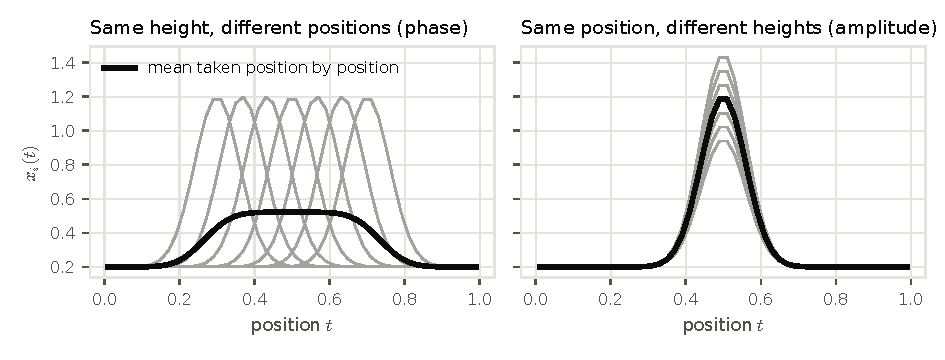
\includegraphics[width=\textwidth]{content/technical/figures/fpca_phase.pdf}
  \caption{Phase and amplitude. Left: seven curves with the same peak at different positions, whose mean taken position by position (black) is a low, wide plateau that resembles none of them. Right: seven curves with the peak at one position and different heights, whose mean keeps the shape of the peak. The curves are simulated and are not data from any cohort.}
  \label{fig:tech-fpca-phase}
\end{figure}

Registration addresses this by warping the domain of each curve with a strictly increasing function that keeps the two ends in place \cite{wang2016fda}.
The warp either moves landmarks, such as peaks, to their average position, or brings each curve close to a common template \cite{wang2016fda}.
Landmark registration is the reference method when clear features are present in every curve, but it fails when a landmark is missing or cannot be identified, which is common in noisy curves \cite{wang2016fda}.

When amplitude and phase vary together, the curves alone cannot tell them apart, so the assumptions built into the warp decide what counts as phase \cite{wang2016fda}.
Reading a component correctly therefore requires knowing which phase variation the registration has removed, if any.
Otherwise, a shift in where a feature lies may be read as a change in its size.
